%==============================================================================
%  MATH 231 -- Linear Algebra I (Queens College, Fall 2026)
%  VECTOR UNIT, PART 3 -- Cauchy-Schwarz, Metrics, and Norms
%
%  This is one of three documents covering the vector unit. Section numbering
%  runs CONTINUOUSLY across all three, so that every cross-reference in the
%  unit means the same thing no matter which part it appears in:
%
%      Part 1  MATH231_vectors_1_definition_and_arithmetic  Sections 1-9
%      Part 2  MATH231_vectors_2_dot_product_and_projection Sections 10-12
%      Part 3  MATH231_vectors_3_norms_and_metrics          Sections 13-15
%
%  Hence the \setcounter{section}{12} below: this part opens at Section 13.
%  Definitions and examples are numbered BY SECTION so that they too are unique
%  across the whole unit.  References to Sections 1-12 point into Parts 1-2.
%
%  AUDIENCE: distributed to students.  Keep it free of instructor-facing
%  apparatus -- time budgets, pacing notes, teaching cues.
%
%  SPLIT POINT.  Cauchy-Schwarz was drafted as Section 12.7, inside the
%  projection section; it is promoted here to Section 13, standing on its own.
%  It is the natural hinge: the projection right triangle hands the inequality
%  over directly (a leg is no longer than the hypotenuse, i.e. a shadow is no
%  longer than its object), and everything after it is about norms.
%
%  NOTATION.  Parts 1-2 write the Euclidean norm as ||v|| with no subscript.
%  Section 14 introduces the family ||v||_p and states that the bare ||v||
%  continues to mean ||v||_2 throughout the unit.
%
%  Sec. 15.3 states HOLDER, not "Cauchy-Schwarz with a p-norm".  The naive
%  |<u,v>| <= ||u||_p ||v||_p is FALSE (p = infinity, u = v = [1,1] gives
%  2 <= 1); the exponents must be conjugate, 1/p + 1/q = 1.  Cauchy-Schwarz is
%  p = q = 2, the one exponent that partners with itself.
%
%  Compile with pdflatex (standard TeX Live packages only; uses tikz).
%==============================================================================

\documentclass[11pt]{article}

\usepackage[margin=1in]{geometry}
\usepackage{amsmath,amssymb,amsthm}
\usepackage[dvipsnames]{xcolor}
\usepackage{enumitem}
\usepackage{booktabs}
\usepackage{array}
\usepackage[hidelinks]{hyperref}
\usepackage{titlesec}
\usepackage{needspace}
\usepackage{tikz}
\usetikzlibrary{arrows.meta}

%------------------------------------------------------------------ style ----
\titleformat{\section}{\large\bfseries\sffamily}{\thesection.}{0.6em}{}
\titleformat{\subsection}{\normalsize\bfseries\sffamily}{\thesubsection.}{0.5em}{}
\titlespacing*{\section}{0pt}{14pt}{6pt}

\theoremstyle{definition}
\newtheorem{defn}{Definition}[section]
\newtheorem{ex}{Example}[section]
\theoremstyle{remark}
\newtheorem*{rmk}{Remark}
\newtheorem*{warn}{A common confusion}

% Honest forward references: things we are simplifying on purpose today and
% will come back to later in the course.
\newcommand{\lookahead}{\par\smallskip\noindent
  \textbf{\sffamily\textcolor{RoyalBlue}{Looking ahead.}}\ \ignorespaces}

%--------------------------------------------------------------- notation ----
\newcommand{\R}{\mathbb{R}}
\newcommand{\vc}[1]{\mathbf{#1}}
\newcommand{\norm}[1]{\lVert #1\rVert}
\newcommand{\uv}[1]{\hat{\vc{#1}}}                 % normalized vector
\newcommand{\Sph}[1]{\mathbb{S}^{#1}}              % the #1-sphere
\newcommand{\proj}[2]{\operatorname{proj}_{#1}(#2)}
\newcommand{\comp}[2]{\operatorname{comp}_{#1}(#2)}

%------------------------------------------------------------- tikz helpers --
\tikzset{
  vecarr/.style   = {-{Stealth[length=2.6mm,width=2.0mm]},very thick},
  thinarr/.style  = {-{Stealth[length=2.2mm,width=1.7mm]},thick},
  axisline/.style = {->,gray!75,thin}
}
% \lattice{xmin}{xmax}{ymin}{ymax}
\newcommand{\lattice}[4]{%
  \draw[step=1cm,gray!25,very thin] (#1,#3) grid (#2,#4);
  \draw[axisline] (#1,0) -- (#2+0.45,0) node[right,font=\scriptsize,black]{$x$};
  \draw[axisline] (0,#3) -- (0,#4+0.45) node[above,font=\scriptsize,black]{$y$};
}
% bare axes, for the small orientation panels
\newcommand{\baxes}[4]{%
  \draw[axisline] (#1,0) -- (#2,0);
  \draw[axisline] (0,#3) -- (0,#4);
}


\title{\vspace{-1.2cm}\textbf{\sffamily MATH 231 -- Linear Algebra I}\\[4pt]
       {\large\sffamily The Vector Unit, Part 3 \textbullet\ Cauchy--Schwarz,
        Metrics, and Norms}\\[2pt]
       {\normalsize\sffamily Kiely Hall 326 \textbullet\
        Instructor: Kevin Bedoya}}
\author{}
\date{}

\begin{document}
\setcounter{section}{12}  % this part opens at Section 13; see the header note
\maketitle
\vspace{-1.6cm}

\noindent\textbf{About this document.} This is Part 3 of the vector unit.
Section numbering runs continuously through all three parts, so a reference such
as \S12.6 points into Part 2 and means exactly what it says:

\begin{center}
\renewcommand{\arraystretch}{1.2}
\begin{tabular}{@{}l l l@{}}
\toprule
\textbf{Part} & \textbf{Sections} & \textbf{Subject} \\
\midrule
1 & \S1--\S9   & vectors, notation, addition, scaling, equality \\
2 & \S10--\S12 & orientation, the dot product, projection \\
3 & \S13--\S15 & Cauchy--Schwarz, metrics, norms \\
\bottomrule
\end{tabular}
\end{center}

\noindent\textbf{Assumed from Parts 1--2.} The Euclidean norm and the scaling
rule $\norm{\alpha\vc{v}}=\lvert\alpha\rvert\norm{\vc{v}}$ (\S8); the triangle
inequality $\norm{\vc{u}+\vc{v}}\le\norm{\vc{u}}+\norm{\vc{v}}$ (\S7.2); the
dot product and $\langle\vc{u},\vc{u}\rangle=\norm{\vc{u}}^{2}$ (\S11); the
angle $\theta\in[0,\pi]$ between two vectors (\S10.3); and the projection
$\proj{\vc{u}}{\vc{v}}$ with its component $\comp{\vc{u}}{\vc{v}}$ (\S12.4).

\medskip
\noindent\textbf{What you should be able to do afterwards.} State the
Cauchy--Schwarz inequality and prove it two ways; list the axioms a metric must
satisfy and verify them for the Euclidean distance; compute Manhattan and
Chebyshev distances; explain why the $1$-, $2$- and $\infty$-norms carry those
subscripts, and derive the $\infty$ case as a limit; state the three properties
that define a norm; and state H\"older's inequality and recognise
Cauchy--Schwarz as its self-conjugate case.

\medskip
\noindent\textbf{Further reading.}
Boyd \& Vandenberghe, \emph{Introduction to Applied Linear Algebra}, Ch.~3
(norm and distance);
Axler, \emph{Linear Algebra Done Right}, Ch.~6 (Cauchy--Schwarz);
Trefethen \& Bau, \emph{Numerical Linear Algebra}, Lec.~3 (norms).

%==============================================================================
\section{The Cauchy--Schwarz inequality}
%==============================================================================
The projection picture has one more thing to tell us, and it is a bound on the
dot product itself.

Look again at the right triangle of \S12.3. Its hypotenuse is $\vc{v}$, with
length $\norm{\vc{v}}$, and one of its legs is the shadow, with length
$\lvert\comp{\vc{u}}{\vc{v}}\rvert$. A leg of a right triangle is never longer
than the hypotenuse --- equivalently, and more memorably:

\begin{quote}
A shadow is never longer than the object casting it.
\end{quote}

\noindent In symbols, $\lvert\comp{\vc{u}}{\vc{v}}\rvert\le\norm{\vc{v}}$. Now
substitute the definition of the component and clear the denominator:
\[
  \left\lvert\frac{\langle\vc{u},\vc{v}\rangle}{\norm{\vc{u}}}\right\rvert
  \;\le\; \norm{\vc{v}}
  \qquad\Longrightarrow\qquad
  \lvert\langle\vc{u},\vc{v}\rangle\rvert \;\le\; \norm{\vc{u}}\,\norm{\vc{v}} .
\]
That is a bound on how large a dot product can possibly be, in terms of nothing
but the two magnitudes --- and it is famous enough to carry two names.

\begin{quote}
\textbf{Cauchy--Schwarz inequality.} For all $\vc{u},\vc{v}\in\R^{2}$,
\[
  \bigl\lvert\langle\vc{u},\vc{v}\rangle\bigr\rvert
  \;\le\;
  \norm{\vc{u}}\,\norm{\vc{v}} .
\]
\end{quote}

\noindent There is also a one-line route to it from \S11 that requires no
picture at all. Since $\langle\vc{u},\vc{v}\rangle=\norm{\vc{u}}\norm{\vc{v}}\cos\theta$
and $\lvert\cos\theta\rvert\le1$ for every angle,
\[
  \bigl\lvert\langle\vc{u},\vc{v}\rangle\bigr\rvert
  = \norm{\vc{u}}\,\norm{\vc{v}}\,\lvert\cos\theta\rvert
  \le \norm{\vc{u}}\,\norm{\vc{v}} .
\]
This second route also settles when the bound is \emph{tight}: equality needs
$\lvert\cos\theta\rvert=1$, hence $\theta=0$ or $\theta=\pi$. So the dot product
attains its largest possible size exactly when the two vectors are parallel or
antiparallel --- when, in the shadow picture, the triangle has collapsed and
$\vc{v}$ lies flat along $\vc{u}$, casting a shadow as long as itself.

\begin{ex}[The bound in action]
For $\vc{u}=[\,3,\,1\,]$ and $\vc{v}=[\,1,\,3\,]$ we found
$\langle\vc{u},\vc{v}\rangle=6$ in \S11, while
$\norm{\vc{u}}\norm{\vc{v}}=\sqrt{10}\cdot\sqrt{10}=10$. And $6\le10$, with
room to spare --- the slack is exactly the factor $\cos\theta=0.6$. For
$\vc{u}=[\,1,\,2\,]$ and $\vc{v}=[\,2,\,4\,]$, which are parallel, we get
$\langle\vc{u},\vc{v}\rangle=10$ and
$\norm{\vc{u}}\norm{\vc{v}}=\sqrt5\cdot2\sqrt5=10$: equality, as predicted.
\end{ex}

\begin{rmk}[Why it matters more than it looks]
Cauchy--Schwarz is what makes \S11.4 legitimate. We defined
$\cos(\vc{u},\vc{v})=\langle\vc{u},\vc{v}\rangle/(\norm{\vc{u}}\norm{\vc{v}})$
and asserted that the output lands in $[-1,1]$ --- but rearrange the inequality
and that assertion \emph{is} Cauchy--Schwarz:
\[
  \bigl\lvert\langle\vc{u},\vc{v}\rangle\bigr\rvert\le\norm{\vc{u}}\norm{\vc{v}}
  \qquad\Longleftrightarrow\qquad
  -1 \;\le\; \frac{\langle\vc{u},\vc{v}\rangle}{\norm{\vc{u}}\,\norm{\vc{v}}} \;\le\; 1 .
\]
In $\R^{2}$ we could lean on the angle $\theta$, which we can see. In higher
dimensions, and in the abstract inner-product spaces of later chapters, there is
no picture to look at and the angle is \emph{defined} by that quotient --- so
something has to guarantee the quotient is a legal cosine before $\arccos$ may
be applied to it. Cauchy--Schwarz is that guarantee, which is why it is stated
as an inequality about inner products rather than as a fact about triangles.
\end{rmk}

\begin{rmk}[A second dividend: the triangle inequality, again]
In \S7.2 we accepted $\norm{\vc{u}+\vc{v}}\le\norm{\vc{u}}+\norm{\vc{v}}$
because a triangle cannot have one side longer than the other two combined ---
true, but geometric. It now follows algebraically. Expanding as in \S11.2,
\[
  \norm{\vc{u}+\vc{v}}^{2}
  = \norm{\vc{u}}^{2}+2\langle\vc{u},\vc{v}\rangle+\norm{\vc{v}}^{2}
  \;\le\; \norm{\vc{u}}^{2}+2\norm{\vc{u}}\norm{\vc{v}}+\norm{\vc{v}}^{2}
  = \bigl(\norm{\vc{u}}+\norm{\vc{v}}\bigr)^{2},
\]
where the middle step is Cauchy--Schwarz. Taking square roots of both
non-negative sides gives the triangle inequality. The geometric picture and the
algebraic bound were the same statement all along.
\end{rmk}

%==============================================================================
\section{Metrics, and the family of norms}
%==============================================================================
Every norm we have written so far has been the Euclidean one, and we have been
writing it $\norm{\vc{v}}$ with no further comment. It is time to admit that
this was a choice. Behind the norm sits a more primitive object --- a notion of
\emph{distance} --- and the Euclidean notion is only one of many.

%------------------------------------------------------------------------------
\subsection{Metrics}
%------------------------------------------------------------------------------
\begin{defn}[Metric]
Let $A$ be a set. A \textbf{metric} on $A$ is a function $d$ that takes two
elements of $A$ and returns a non-negative real number --- interpreted as the
\emph{distance} between them --- subject to the following. For all
$x,y,z\in A$:
\begin{enumerate}[label=\textbf{M\arabic*.},leftmargin=3.0em,itemsep=4pt,
                  topsep=4pt]
  \item $d(x,y)=0 \iff x=y$
        \hfill (a point is at distance zero from itself, and from nothing else)
  \item $d(x,y)=d(y,x)$
        \hfill (symmetry)
  \item $d(x,y)+d(y,z)\ge d(x,z)$
        \hfill (triangle inequality)
  \item $d(x,y)\ge 0$
        \hfill (non-negativity)
\end{enumerate}
\end{defn}

\noindent The elements of $A$ are usually points of a coordinate space --- for
us $A=\R^{2}$, and the two elements are two vectors --- but nothing in the
definition requires that. Metrics are defined on sets of strings, of functions,
of images, of DNA sequences. The four conditions are all that ``distance'' has
to mean.

\begin{rmk}
Axiom \textbf{M4} is listed for emphasis, but it is not independent: it follows
from the other three. Put $z=x$ in \textbf{M3} to get
$d(x,y)+d(y,x)\ge d(x,x)$, which is $0$ by \textbf{M1}. Then \textbf{M2} turns
the left side into $2d(x,y)$, so $2d(x,y)\ge 0$ and hence $d(x,y)\ge 0$. Worth
knowing, because it means that to check something is a metric you only ever have
to check three things.
\end{rmk}

%------------------------------------------------------------------------------
\subsection{The Euclidean distance is a metric}
%------------------------------------------------------------------------------
The distance we have been using all along is
\[
  d_2(\vc{x},\vc{y})
  \;=\; \sqrt{(x_1-y_1)^{2}+(x_2-y_2)^{2}}
  \;=\; \norm{\vc{x}-\vc{y}} ,
\]
the norm of the difference --- which is exactly the between-the-heads reading of
\S7.3. Let us check all four axioms. Each one turns out to be a result we
already have.

\smallskip
\noindent\textbf{M1.} Suppose $d_2(\vc{x},\vc{y})=0$. Then
$(x_1-y_1)^{2}+(x_2-y_2)^{2}=0$. A sum of two squares of real numbers is zero
only if each square is zero, so $x_1=y_1$ and $x_2=y_2$ --- that is,
$\vc{x}=\vc{y}$ by the equality of \S9. Conversely, if $\vc{x}=\vc{y}$ then both
differences vanish and the square root is $0$. \hfill$\checkmark$

\smallskip
\noindent\textbf{M2.} Since $\vc{x}-\vc{y}=-(\vc{y}-\vc{x})$, the scaling rule
of \S8 with $\alpha=-1$ gives
\[
  \norm{\vc{x}-\vc{y}}
  = \norm{(-1)(\vc{y}-\vc{x})}
  = \lvert -1\rvert\,\norm{\vc{y}-\vc{x}}
  = \norm{\vc{y}-\vc{x}} ,
\]
so $d_2(\vc{x},\vc{y})=d_2(\vc{y},\vc{x})$. Geometrically: mirroring a
displacement does not change its length. \hfill$\checkmark$

\smallskip
\noindent\textbf{M3.} This is \S7.2 in disguise. Put
$\vc{u}=\vc{x}-\vc{y}$ and $\vc{v}=\vc{y}-\vc{z}$, and notice that
\[
  \vc{u}+\vc{v} = (\vc{x}-\vc{y})+(\vc{y}-\vc{z}) = \vc{x}-\vc{z} .
\]
The triangle inequality for norms says $\norm{\vc{u}+\vc{v}}\le
\norm{\vc{u}}+\norm{\vc{v}}$, which reads
\[
  \norm{\vc{x}-\vc{z}} \;\le\; \norm{\vc{x}-\vc{y}}+\norm{\vc{y}-\vc{z}},
  \qquad\text{that is}\qquad
  d_2(\vc{x},\vc{z}) \le d_2(\vc{x},\vc{y})+d_2(\vc{y},\vc{z}) .
\]
\hfill$\checkmark$

\smallskip
\noindent\textbf{M4.} A square root of a non-negative quantity is
non-negative. \hfill$\checkmark$

\begin{rmk}
Notice what \textbf{M3} explains retroactively. In \S7.2 we called
$\norm{\vc{u}+\vc{v}}\le\norm{\vc{u}}+\norm{\vc{v}}$ the ``triangle
inequality'' because of a picture of a triangle. We can now see the deeper
reason for the name: it is the axiom that makes distance behave like distance,
in \emph{any} setting, with or without a picture.
\end{rmk}

%------------------------------------------------------------------------------
\subsection{A different geometry: the Manhattan metric}
%------------------------------------------------------------------------------
The Euclidean metric assigns to two points the length of the shortest straight
line joining them. That is humanity's most familiar notion of distance, and in
flat coordinate space it is the right one. But ``shortest path'' depends on which
paths are \emph{available}, and that depends on the geometry of the space you are
moving through.

So consider a plane carved into a grid of city blocks by streets and avenues,
and suppose you must travel between two street corners. You are not allowed to
cut through the buildings. Every route is a sequence of moves along streets and
avenues, and the Euclidean distance --- the straight line between the corners
--- is not merely inconvenient but \emph{wrong}: it would report the distance
you could travel if you could pass through walls, which badly understates the
trip.

What is the honest answer? Any legal route must cover the whole horizontal gap
and the whole vertical gap, and no route need cover more. So the distance is the
sum of the two gaps, and it does not matter in what order you take them.

\begin{defn}[Manhattan metric]
For $\vc{x}=(x_1,x_2)$ and $\vc{y}=(y_1,y_2)$ in $\R^{2}$, the
\textbf{Manhattan} or \textbf{taxicab} metric is
\[
  d_1(\vc{x},\vc{y}) \;=\; \lvert x_1-y_1\rvert + \lvert x_2-y_2\rvert .
\]
\end{defn}

\noindent The name is as literal as it sounds: it is the distance a taxi drives
on a rectangular street grid.

\smallskip
\noindent\emph{Exercise (homework).} Verify that $d_1$ satisfies
\textbf{M1}--\textbf{M3}, and hence is a metric on $\R^{2}$.

\subsubsection*{Practice}
\begin{enumerate}[label=\textbf{P\arabic*.},leftmargin=2.8em,itemsep=5pt,
                  topsep=5pt]
  \item Compute $d_1(\vc{x},\vc{y})$ for $\vc{x}=(1,2)$ and $\vc{y}=(4,6)$.
  \item Compute $d_1(\vc{x},\vc{y})$ for $\vc{x}=(-2,3)$ and $\vc{y}=(3,-1)$.
\end{enumerate}

\smallskip
\noindent\textbf{Answers.}
\begin{align*}
  \text{P1:}\quad d_1 &= \lvert 1-4\rvert+\lvert 2-6\rvert = 3+4 = 7,
    &&\text{compare } d_2=\sqrt{9+16}=5 . \\
  \text{P2:}\quad d_1 &= \lvert -2-3\rvert+\lvert 3-(-1)\rvert = 5+4 = 9,
    &&\text{compare } d_2=\sqrt{25+16}=\sqrt{41}\approx 6.40 .
\end{align*}
In both cases the taxicab distance exceeds the Euclidean one, which is what you
should expect: forbidding diagonal movement can only make the trip longer.

%------------------------------------------------------------------------------
\subsection{The Chebyshev metric}
%------------------------------------------------------------------------------
A third notion of distance keeps only the \emph{largest} of the coordinate
displacements and ignores the other entirely.

\begin{defn}[Chebyshev metric]
For $\vc{x},\vc{y}\in\R^{2}$, the \textbf{Chebyshev} metric is
\[
  d_\infty(\vc{x},\vc{y})
  \;=\; \max\bigl\{\,\lvert x_1-y_1\rvert,\;\lvert x_2-y_2\rvert\,\bigr\}.
\]
\end{defn}

\begin{rmk}[Why it is called the chess metric]
Think of a king on a chessboard. A king moves one square per turn in any of
eight directions, including diagonally --- and a diagonal step advances it by
one square \emph{horizontally and vertically at the same time}. So the smaller
of the two displacements comes for free: it is covered incidentally while
closing the larger one. The number of moves a king needs to travel between two
squares is therefore exactly the larger of the horizontal and vertical gaps ---
precisely $d_\infty$.

For example, from $(1,1)$ to $(4,3)$ the gaps are $3$ and $2$, so
$d_\infty=3$, and indeed three moves suffice:
$(1,1)\to(2,2)\to(3,3)\to(4,3)$. No shorter route exists, because three columns
must be crossed and a king crosses at most one per move.
\end{rmk}

%------------------------------------------------------------------------------
\subsection{Naming the norms}
%------------------------------------------------------------------------------
Each of these metrics has a norm attached to it, and the two are two views of
the same measurement:
\[
  \norm{\vc{v}} = d(\vc{v},\vc{0})
  \qquad\text{and}\qquad
  d(\vc{x},\vc{y}) = \norm{\vc{x}-\vc{y}} .
\]
The norm is the distance from the origin; the distance is the norm of the
difference. So each of our three metrics names a norm, and since there are now
several we can no longer write $\norm{\vc{v}}$ and leave it at that. The
standard fix is a \textbf{subscript}:

\begin{center}
\renewcommand{\arraystretch}{1.6}
\begin{tabular}{@{}l l l@{}}
\toprule
\textbf{Norm} & \textbf{Notation} & \textbf{Formula} \\
\midrule
Manhattan / taxicab & $\norm{\vc{v}}_1$
  & $\lvert v_1\rvert+\lvert v_2\rvert$ \\
Euclidean           & $\norm{\vc{v}}_2$
  & $\sqrt{\lvert v_1\rvert^{2}+\lvert v_2\rvert^{2}}$ \\
Chebyshev           & $\norm{\vc{v}}_\infty$
  & $\max\bigl\{\lvert v_1\rvert,\lvert v_2\rvert\bigr\}$ \\
\bottomrule
\end{tabular}
\end{center}

\begin{rmk}[Our convention]
Everywhere in \S1--\S13, and everywhere later unless a subscript says
otherwise, a bare $\norm{\vc{v}}$ means the Euclidean norm $\norm{\vc{v}}_2$.
The Euclidean norm keeps the privilege of needing no subscript.
\end{rmk}

\noindent Which leaves an obvious question: why $1$, $2$ and $\infty$? The
numbers are not arbitrary labels. They are parameter values.

%------------------------------------------------------------------------------
\subsection{The $p$-norm}
%------------------------------------------------------------------------------
\begin{defn}[$p$-norm]
For a real number $p\ge 1$ and $\vc{v}=[\,v_1,\,v_2\,]\in\R^{2}$, the
\textbf{$p$-norm} of $\vc{v}$ is
\[
  \norm{\vc{v}}_p
  \;=\;
  \bigl(\lvert v_1\rvert^{p}+\lvert v_2\rvert^{p}\bigr)^{1/p} .
\]
\end{defn}

\noindent Two of our three norms are already on this list. Setting $p=1$,
\[
  \norm{\vc{v}}_1
  = \bigl(\lvert v_1\rvert^{1}+\lvert v_2\rvert^{1}\bigr)^{1/1}
  = \lvert v_1\rvert+\lvert v_2\rvert ,
\]
which is the Manhattan norm. Setting $p=2$,
\[
  \norm{\vc{v}}_2
  = \bigl(\lvert v_1\rvert^{2}+\lvert v_2\rvert^{2}\bigr)^{1/2}
  = \sqrt{v_1^{2}+v_2^{2}} ,
\]
which is the Euclidean norm --- the absolute values are harmless here, since
squaring destroys signs anyway. So the subscripts were never names; they were
\emph{the value of $p$}. This is why the Manhattan and Euclidean norms are
properly called the \textbf{$1$-norm} and the \textbf{$2$-norm}.

\begin{rmk}[Why $p\ge 1$]
The restriction is not decoration --- the formula stops being a norm below $1$.
Take $p=\tfrac12$, $\vc{u}=[\,1,\,0\,]$ and $\vc{v}=[\,0,\,1\,]$. Then
$\norm{\vc{u}}_{1/2}=1^{2}=1$ and $\norm{\vc{v}}_{1/2}=1$, while
$\vc{u}+\vc{v}=[\,1,\,1\,]$ gives
\[
  \norm{\vc{u}+\vc{v}}_{1/2} = \bigl(1+1\bigr)^{2} = 4 .
\]
But $4>1+1$, so the triangle inequality fails. Whatever that formula measures,
it is not a length.
\end{rmk}

%------------------------------------------------------------------------------
\subsection{What happens as \texorpdfstring{$p\to\infty$}{p to infinity}}
%------------------------------------------------------------------------------
That accounts for $1$ and $2$. But the Chebyshev norm was defined by a
\emph{maximum}, which looks nothing like the $p$-norm formula --- and its
subscript is not even a number. Both puzzles are resolved by the same
computation.

\begin{quote}
\textbf{Claim.} For every $\vc{v}\in\R^{2}$,
\[
  \lim_{p\to\infty}\norm{\vc{v}}_p
  \;=\;
  \max\bigl\{\lvert v_1\rvert,\lvert v_2\rvert\bigr\} .
\]
\end{quote}

\noindent\emph{Proof.} If $\vc{v}=\vc{0}$ both sides are $0$, so assume
$\vc{v}\neq\vc{0}$ and write
\[
  M = \max\bigl\{\lvert v_1\rvert,\lvert v_2\rvert\bigr\} > 0 .
\]
The idea is to trap $\norm{\vc{v}}_p$ between two quantities that both approach
$M$, and then apply the squeeze theorem from MATH~141.

\smallskip
\noindent\textbf{A lower bound.} One of the two coordinates realises the
maximum, so one of the terms $\lvert v_1\rvert^{p}$, $\lvert v_2\rvert^{p}$
equals $M^{p}$ exactly. The other term is non-negative. Hence
\[
  \lvert v_1\rvert^{p}+\lvert v_2\rvert^{p} \;\ge\; M^{p},
\]
and raising both sides to the power $1/p$ --- which preserves the inequality,
since $t\mapsto t^{1/p}$ is increasing on $[0,\infty)$ ---
\[
  \norm{\vc{v}}_p \;\ge\; \bigl(M^{p}\bigr)^{1/p} = M .
\]

\smallskip
\noindent\textbf{An upper bound.} Every coordinate is at most $M$ in absolute
value, so each term is at most $M^{p}$, and there are two of them:
\[
  \lvert v_1\rvert^{p}+\lvert v_2\rvert^{p} \;\le\; 2M^{p} .
\]
Again taking $p$-th roots,
\[
  \norm{\vc{v}}_p \;\le\; \bigl(2M^{p}\bigr)^{1/p} = 2^{1/p}\,M .
\]

\smallskip
\noindent\textbf{Squeezing.} Combining the two bounds, for every $p\ge1$,
\[
  M \;\le\; \norm{\vc{v}}_p \;\le\; 2^{1/p}\,M .
\]
Now let $p\to\infty$. The left-hand bound does not depend on $p$ at all, so it
stays at $M$. On the right, $1/p\to0$ and $t\mapsto 2^{t}$ is continuous, so
$2^{1/p}\to 2^{0}=1$ and the whole bound tends to $M$. Both outer quantities
converge to the same limit $M$, so by the squeeze theorem the quantity trapped
between them does too:
\[
  \lim_{p\to\infty}\norm{\vc{v}}_p = M
  = \max\bigl\{\lvert v_1\rvert,\lvert v_2\rvert\bigr\}. \qquad\blacksquare
\]

\noindent Both puzzles dissolve at once. The Chebyshev norm is not a separate
construction bolted on beside the others --- it is the \emph{limiting case} of
the $p$-norm family, which is exactly why its subscript is $\infty$:
\[
  \norm{\vc{v}}_\infty := \lim_{p\to\infty}\norm{\vc{v}}_p
  = \max\bigl\{\lvert v_1\rvert,\lvert v_2\rvert\bigr\}.
\]
And the maximum was inevitable. As $p$ grows, raising to the $p$-th power
exaggerates the gap between a larger and a smaller number without limit, so the
larger coordinate comes to dominate the sum completely and the smaller one
becomes negligible. Taking $p\to\infty$ makes that domination total.

\begin{rmk}
Nothing in the argument used the fact that there are exactly two coordinates.
In $\R^{n}$ the upper bound becomes $n^{1/p}M$, and $n^{1/p}\to1$ just as
$2^{1/p}$ did --- the constant is different, the limit is not. All that matters
is that the number of coordinates is finite.
\end{rmk}

%------------------------------------------------------------------------------
\subsection{Unit balls: the shape of ``length one''}
%------------------------------------------------------------------------------
In \S12.1 we found that the vectors of unit length trace a circle of radius $1$,
and flagged that this was an artefact of the Euclidean norm. Now we can see what
the other norms give. In each case we are drawing the same set --- the vectors
whose length is $1$ --- under a different definition of length.

\begin{itemize}[leftmargin=1.4em,itemsep=4pt]
  \item $\norm{\vc{v}}_1=1$ means $\lvert v_1\rvert+\lvert v_2\rvert=1$. In the
        first quadrant that is the line $v_1+v_2=1$ joining $(1,0)$ to $(0,1)$;
        reflecting into the other three quadrants gives a \textbf{diamond} with
        vertices at $(\pm1,0)$ and $(0,\pm1)$.
  \item $\norm{\vc{v}}_2=1$ means $v_1^{2}+v_2^{2}=1$: the \textbf{circle} of
        radius $1$.
  \item $\norm{\vc{v}}_\infty=1$ means the larger of $\lvert v_1\rvert$,
        $\lvert v_2\rvert$ equals $1$ while the other is at most $1$: the
        boundary of the \textbf{square} with corners $(\pm1,\pm1)$.
\end{itemize}

\noindent All three are centred at the origin. The set is called the
\emph{unit ball} of the norm, and its shape is the norm's signature.

\begin{center}
\begin{tabular}{@{}c@{\hspace{0.9cm}}c@{\hspace{0.9cm}}c@{}}
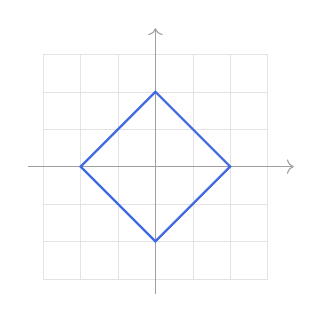
\begin{tikzpicture}[scale=0.95]
  % grid must start on a multiple of the step, or the lines miss the integers
  \draw[step=0.5cm,gray!22,very thin] (-1.5,-1.5) grid (1.5,1.5);
  \draw[axisline] (-1.7,0) -- (1.85,0);
  \draw[axisline] (0,-1.7) -- (0,1.85);
  \draw[RoyalBlue,thick] (1,0) -- (0,1) -- (-1,0) -- (0,-1) -- cycle;
\end{tikzpicture}
&
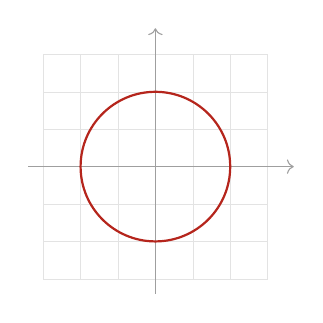
\begin{tikzpicture}[scale=0.95]
  % grid must start on a multiple of the step, or the lines miss the integers
  \draw[step=0.5cm,gray!22,very thin] (-1.5,-1.5) grid (1.5,1.5);
  \draw[axisline] (-1.7,0) -- (1.85,0);
  \draw[axisline] (0,-1.7) -- (0,1.85);
  \draw[BrickRed,thick] (0,0) circle (1);
\end{tikzpicture}
&
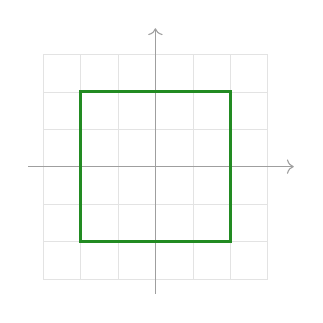
\begin{tikzpicture}[scale=0.95]
  % grid must start on a multiple of the step, or the lines miss the integers
  \draw[step=0.5cm,gray!22,very thin] (-1.5,-1.5) grid (1.5,1.5);
  \draw[axisline] (-1.7,0) -- (1.85,0);
  \draw[axisline] (0,-1.7) -- (0,1.85);
  % heavier stroke: this square's edges lie on gridlines and would blend in
  \draw[ForestGreen,very thick] (-1,-1) rectangle (1,1);
\end{tikzpicture}
\\[3pt]
{\small $\norm{\vc{v}}_1=1$: a diamond} &
{\small $\norm{\vc{v}}_2=1$: a circle} &
{\small $\norm{\vc{v}}_\infty=1$: a square}
\end{tabular}
\end{center}

\subsubsection*{Varying $p$ continuously}
The three pictures are not three unrelated shapes. The $p$-norm is continuous
in $p$, so as $p$ increases from $1$ the unit ball deforms smoothly: the
diamond's flat edges bow outward, passing exactly through the circle at $p=2$,
and continue bulging until they flatten against the square in the limit
$p\to\infty$.

\begin{center}
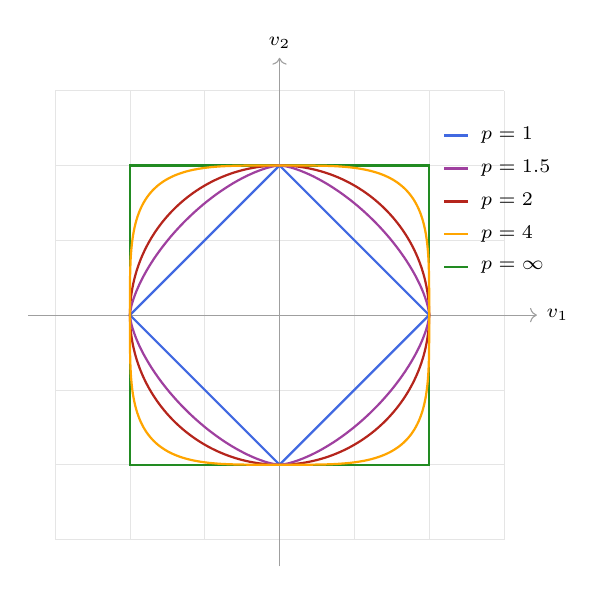
\begin{tikzpicture}[scale=1.9]
  % grid must start on a multiple of the step, or the lines miss the integers
  \draw[step=0.5cm,gray!20,very thin] (-1.5,-1.5) grid (1.5,1.5);
  \draw[axisline] (-1.68,0) -- (1.72,0) node[right,font=\scriptsize,black]{$v_1$};
  \draw[axisline] (0,-1.68) -- (0,1.72) node[above,font=\scriptsize,black]{$v_2$};
  % p = infinity (square) and p = 1 (diamond): exact, drawn as straight lines
  \draw[ForestGreen,thick] (-1,-1) rectangle (1,1);
  \draw[RoyalBlue,thick] (1,0) -- (0,1) -- (-1,0) -- (0,-1) -- cycle;
  % p = 2: exact circle
  \draw[BrickRed,thick] (0,0) circle (1);
  % intermediate p, via the superellipse |cos t|^(2/p), |sin t|^(2/p);
  % the domain is offset so the samples never land exactly on 90/180/270
  \draw[Purple!75,thick,domain=0.7:360.7,smooth,variable=\t,samples=200]
        plot ({sign(cos(\t))*(abs(cos(\t)))^(2/1.5)},
              {sign(sin(\t))*(abs(sin(\t)))^(2/1.5)});
  \draw[Orange,thick,domain=0.7:360.7,smooth,variable=\t,samples=200]
        plot ({sign(cos(\t))*(abs(cos(\t)))^(2/4)},
              {sign(sin(\t))*(abs(sin(\t)))^(2/4)});
  % legend: a short stroke in each colour, keyed to the curves above
  \draw[RoyalBlue,thick]   (1.10,1.20) -- (1.26,1.20);
  \draw[Purple!75,thick]   (1.10,0.98) -- (1.26,0.98);
  \draw[BrickRed,thick]    (1.10,0.76) -- (1.26,0.76);
  \draw[Orange,thick]      (1.10,0.54) -- (1.26,0.54);
  \draw[ForestGreen,thick] (1.10,0.32) -- (1.26,0.32);
  \node[right,font=\scriptsize] at (1.28,1.20) {$p=1$};
  \node[right,font=\scriptsize] at (1.28,0.98) {$p=1.5$};
  \node[right,font=\scriptsize] at (1.28,0.76) {$p=2$};
  \node[right,font=\scriptsize] at (1.28,0.54) {$p=4$};
  \node[right,font=\scriptsize] at (1.28,0.32) {$p=\infty$};
\end{tikzpicture}
\end{center}

\noindent Reading the picture from the inside out also reveals an ordering. The
diamond sits inside the circle, which sits inside the square, and the balls only
ever grow as $p$ grows. Since a \emph{larger} unit ball means it takes a bigger
vector to reach length $1$, the norms themselves run the other way:
\[
  \norm{\vc{v}}_\infty \;\le\; \norm{\vc{v}}_2 \;\le\; \norm{\vc{v}}_1 .
\]
Check it on $\vc{v}=[\,1,\,1\,]$: the three norms are $1$, $\sqrt2\approx1.414$,
and $2$. The same vector has three different lengths, and which one is
``correct'' is a question about the problem you are solving, not about the
vector.

\lookahead We have now met four metrics and a whole family of norms, but we have
not yet said what a \emph{norm} is in the way that \S14.1 said what a metric is
--- the $p\ge1$ restriction, for instance, was justified by one counterexample
rather than by a definition. The next section gives the axioms a norm must
satisfy and checks them against the family we have built.

%==============================================================================
\section{What makes a norm a norm}
%==============================================================================
Section~13 built an entire family of norms without ever saying what the word
means. A \textbf{norm} is a function that takes a vector and returns a
non-negative real number,
\[
  \norm{\,\cdot\,}\;:\;\R^{2}\to\R ,
\]
subject to three conditions. Every member of the $p$-norm family satisfies them,
for every $p$ in $[1,\infty)$ --- and so does the limiting case $p=\infty$.

%------------------------------------------------------------------------------
\subsection{The three properties}
%------------------------------------------------------------------------------
\begin{quote}
For all $\vc{u},\vc{v}\in\R^{2}$ and all $\alpha\in\R$:

\smallskip
\textbf{N1. Positive definiteness.}
\[
  \norm{\vc{v}}\ge 0,
  \qquad\text{and}\qquad
  \norm{\vc{v}}=0 \iff \vc{v}=\vc{0}.
\]

\smallskip
\textbf{N2. Absolute homogeneity.}
\[
  \norm{\alpha\vc{v}} = \lvert\alpha\rvert\,\norm{\vc{v}} .
\]

\smallskip
\textbf{N3. Triangle inequality} (also called \emph{subadditivity}).
\[
  \norm{\vc{u}+\vc{v}} \;\le\; \norm{\vc{u}}+\norm{\vc{v}} .
\]
\end{quote}

\noindent None of these should be new. \textbf{N2} is the scaling rule we
established in \S8 --- the size $\lvert\alpha\rvert$ sets the length and the sign
is discarded, which is exactly why the absolute value appears. \textbf{N3} is
\S7.2, first justified by a triangle and later derived from Cauchy--Schwarz in
\S13. What \S15 adds is the recognition that these are not three assorted
facts about the Euclidean norm; they are the \emph{definition} of length, and any
function satisfying them earns the name.

\begin{rmk}[Which parts are doing real work]
Exactly as with the metric axioms of \S14.1, the list is not minimal.
Homogeneity with $\alpha=0$ gives $\norm{\vc{0}}=\lvert 0\rvert\norm{\vc{v}}=0$,
so half of \textbf{N1} is free. And non-negativity follows from the other two:
\[
  0 = \norm{\vc{0}} = \norm{\vc{v}+(-\vc{v})}
    \le \norm{\vc{v}}+\norm{-\vc{v}}
    = \norm{\vc{v}}+\lvert-1\rvert\norm{\vc{v}}
    = 2\norm{\vc{v}} ,
\]
so $\norm{\vc{v}}\ge0$. What cannot be derived, and is therefore the real
content of \textbf{N1}, is the converse direction: $\norm{\vc{v}}=0$ forces
$\vc{v}=\vc{0}$. Drop it and the function sending \emph{every} vector to $0$
would qualify as a norm --- it satisfies \textbf{N2} and \textbf{N3} perfectly.
That is why the property is called positive \emph{definiteness} rather than
merely non-negativity: it is the clause that stops a norm from collapsing.
\end{rmk}

%------------------------------------------------------------------------------
\subsection{The family passes}
%------------------------------------------------------------------------------
Two of the three are quick to confirm for every $p$ at once.

\smallskip
\noindent\textbf{N1.} $\norm{\vc{v}}_p=0$ forces
$\lvert v_1\rvert^{p}+\lvert v_2\rvert^{p}=0$. That is a sum of two
non-negative numbers, so both vanish, so $v_1=v_2=0$. \hfill$\checkmark$

\smallskip
% keep the statement, the display, and its tick mark on one page
\Needspace*{8\baselineskip}
\noindent\textbf{N2.} Pull the scalar out one coordinate at a time:
\[
  \norm{\alpha\vc{v}}_p
  = \bigl(\lvert\alpha v_1\rvert^{p}+\lvert\alpha v_2\rvert^{p}\bigr)^{1/p}
  = \bigl(\lvert\alpha\rvert^{p}
     \bigl(\lvert v_1\rvert^{p}+\lvert v_2\rvert^{p}\bigr)\bigr)^{1/p}
  = \lvert\alpha\rvert
     \bigl(\lvert v_1\rvert^{p}+\lvert v_2\rvert^{p}\bigr)^{1/p}
  = \lvert\alpha\rvert\,\norm{\vc{v}}_p .
\]
\hfill$\checkmark$

\smallskip
\noindent\textbf{N3} is the hard one, and it is precisely where the restriction
$p\ge1$ earns its keep --- recall the $p=\tfrac12$ counterexample of \S14.6. The
two ends of the family are easy. For $p=1$, apply the scalar inequality
$\lvert a+b\rvert\le\lvert a\rvert+\lvert b\rvert$ in each coordinate:
\[
  \norm{\vc{u}+\vc{v}}_1
  = \lvert u_1+v_1\rvert+\lvert u_2+v_2\rvert
  \le \lvert u_1\rvert+\lvert v_1\rvert+\lvert u_2\rvert+\lvert v_2\rvert
  = \norm{\vc{u}}_1+\norm{\vc{v}}_1 .
\]
For $p=\infty$, the same scalar inequality inside a maximum:
\[
  \norm{\vc{u}+\vc{v}}_\infty
  = \max_i\lvert u_i+v_i\rvert
  \le \max_i\bigl(\lvert u_i\rvert+\lvert v_i\rvert\bigr)
  \le \max_i\lvert u_i\rvert+\max_i\lvert v_i\rvert
  = \norm{\vc{u}}_\infty+\norm{\vc{v}}_\infty .
\]
For $p$ strictly between, the inequality is a genuine theorem with a name ---
\textbf{Minkowski's inequality} --- whose proof needs machinery beyond this
course. We will use it, and record that it holds for every $p\ge1$ and fails for
every $p<1$.

%------------------------------------------------------------------------------
\subsection{Cauchy--Schwarz, generalised}
%------------------------------------------------------------------------------
In \S13 we proved
$\lvert\langle\vc{u},\vc{v}\rangle\rvert\le\norm{\vc{u}}\norm{\vc{v}}$, with both
norms Euclidean. Now that other norms exist, the natural question is what
replaces it.

\begin{rmk}[The obvious guess is false]
One might hope for
$\lvert\langle\vc{u},\vc{v}\rangle\rvert\le\norm{\vc{u}}_p\norm{\vc{v}}_p$ with
the \emph{same} $p$ on both factors. Test it at $p=\infty$ with
$\vc{u}=\vc{v}=[\,1,\,1\,]$: then $\langle\vc{u},\vc{v}\rangle=2$, while
$\norm{\vc{u}}_\infty\norm{\vc{v}}_\infty=1\cdot1=1$. The bound would claim
$2\le1$. So the two exponents cannot be equal in general.
\end{rmk}

\noindent The correct statement pairs each exponent with a partner.

\begin{quote}
\textbf{H\"older's inequality.} Let $p,q\ge1$ satisfy
\[
  \frac{1}{p}+\frac{1}{q} = 1 .
\]
Then for all $\vc{u},\vc{v}\in\R^{2}$,
\[
  \bigl\lvert\langle\vc{u},\vc{v}\rangle\bigr\rvert
  \;\le\; \norm{\vc{u}}_p\,\norm{\vc{v}}_q .
\]
\end{quote}

\noindent Such a $p$ and $q$ are called \textbf{conjugate exponents}. Three
pairings matter in practice:
\[
  (p,q)=(2,2), \qquad (p,q)=(1,\infty), \qquad (p,q)=(\infty,1),
\]
where the convention $1/\infty=0$ makes the middle two legitimate. And notice
the first: $\tfrac12+\tfrac12=1$, so $p=q=2$ is conjugate to itself, and
H\"older reads
\[
  \bigl\lvert\langle\vc{u},\vc{v}\rangle\bigr\rvert
  \le \norm{\vc{u}}_2\,\norm{\vc{v}}_2 ,
\]
which is Cauchy--Schwarz exactly. So Cauchy--Schwarz was never a standalone
result; it is the self-conjugate case of a family, and the reason it looks
symmetric is that $2$ is the one exponent that partners with itself. Re-running
the failed example above with the correct pairing $(\infty,1)$ gives
$\norm{\vc{u}}_\infty\norm{\vc{v}}_1=1\cdot2=2$, and $2\le2$ holds --- with
equality.

%------------------------------------------------------------------------------
\subsection{Norms beyond \texorpdfstring{$\R^{2}$}{R2}: quaternions}
%------------------------------------------------------------------------------
Nothing in \textbf{N1}--\textbf{N3} mentioned the dimension, or even that the
objects were arrows in a plane. Anything with a sensible notion of addition and
scaling can carry a norm. The quaternions of the complex numbers lecture are a
convenient example: a quaternion
\[
  q = a+bi+cj+dk
\]
carries four real numbers, so it behaves like a vector in $\R^{4}$, and its
modulus is the Euclidean norm of that $4$-vector:
\[
  \lvert q\rvert = \sqrt{a^{2}+b^{2}+c^{2}+d^{2}}
  = \bigl\lVert [\,a,\,b,\,c,\,d\,]\bigr\rVert_2 .
\]
All three properties come for free, because it \emph{is} a Euclidean norm: a sum
of four squares vanishes only when every term does (\textbf{N1}), a real scalar
factors out in absolute value (\textbf{N2}), and \textbf{N3} is the triangle
inequality in $\R^{4}$.

\begin{ex}
For $q=1+i+j+k$, $\lvert q\rvert=\sqrt{1+1+1+1}=2$. For $q=3+4i$ --- a complex
number, viewed as a quaternion with $c=d=0$ --- $\lvert q\rvert=\sqrt{9+16}=5$,
agreeing with the modulus we would have computed in $\mathbb{C}$.
\end{ex}

\begin{rmk}[One property vectors do not have]
The quaternion norm is \textbf{multiplicative}:
$\lvert q_1q_2\rvert=\lvert q_1\rvert\lvert q_2\rvert$. Check it on the product
computed in the complex numbers lecture, $q=1+i$ and $p=1+j$, whose product was
$qp=1+i+j+k$:
\[
  \lvert q\rvert\,\lvert p\rvert = \sqrt2\cdot\sqrt2 = 2
  = \lvert 1+i+j+k\rvert = \lvert qp\rvert . \quad\checkmark
\]
No such statement is available for vectors in $\R^{2}$, for the simple reason
that there is nothing to put on the left: two vectors have no product that
returns a vector. Multiplicativity is a property of the extra algebraic
structure, not of the norm.
\end{rmk}

%------------------------------------------------------------------------------
\subsection{Why this matters}
%------------------------------------------------------------------------------
Norms are among the most heavily used operations in computational science, and
they will recur throughout this course --- rarely as an object of study in their
own right, and almost always as the thing being measured, minimised, or bounded.
A norm is how we say that an approximation is close to an answer, that an
algorithm has converged, that an error is small enough to stop, or that one
matrix is nearly another.

\lookahead Three appearances worth anticipating. Least squares is stated as
$\min_{\vc{x}}\norm{A\vc{x}-\vc{b}}_2$ --- a norm being minimised, and the choice
of $p=2$ is exactly what makes the problem solvable by the geometry of \S12.6.
Every iterative method needs a stopping rule of the form ``halt when
$\norm{\text{residual}}$ drops below a tolerance,'' so the norm sets the meaning
of \emph{done}. And the notion of a norm extends from vectors to matrices,
giving the condition number that measures how badly a linear system amplifies
error.

\lookahead A last remark on the unit-ball pictures of \S14.8, which are less
decorative than they look. The $1$-norm's diamond has its corners \emph{on the
axes}, where one coordinate is zero; the $2$-norm's circle has no corners at all.
When a norm is minimised subject to a constraint, solutions tend to land at
corners --- so minimising with $\norm{\cdot}_1$ tends to produce answers with
zero entries, while $\norm{\cdot}_2$ does not. That single geometric difference
is the reason $\ell_1$ penalties are used to force sparse solutions in modern
statistics and machine learning. The shape of the ball is the whole explanation.

\end{document}
